%%%%%%%%%%%%%%%%%%%%%%%%%%%%%%%%%%%%%%%%%%%%%%%%%%%%%%%%%%%%%%%%%%%%%%%%%%%%%%%%
\subsubsection{Homodyne Detection System}

\begin{figure}[ht]
    \centering
    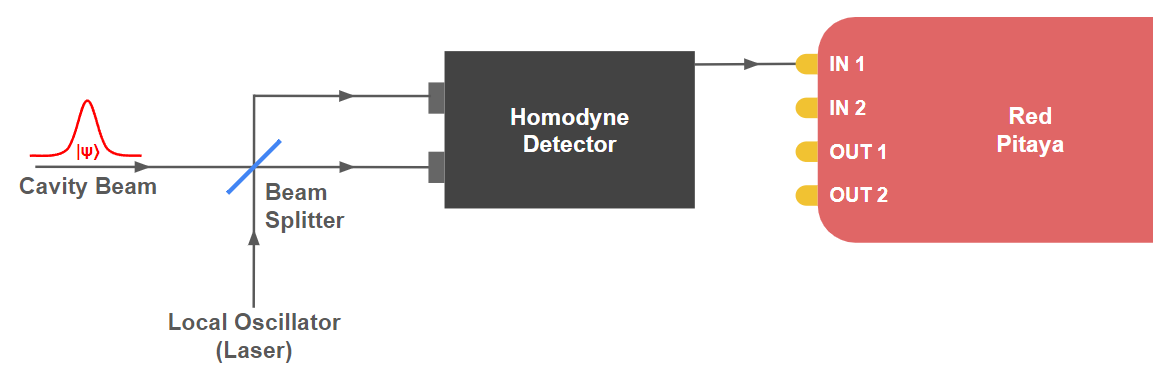
\includegraphics[width=0.9\columnwidth]{images/chapter_2/2_noise/homo_detection.png}
    \caption{Illustration of homodyne detection system in the experimental setup.}
    \label{fig:ch2_homo_detection}
\end{figure}

\noindent Currently, a critical role of the NI 5761 Analog Input module is the acquisition and processing of data by homodyne detection of the beam coming from the cavity in the presence of Rb atoms. Such a cavity beam is a result of the probe and control pulses sent into the cavity. Homodyne detection allows the measurement of a quadrature of the electric field of the input signal \cite{valentin}. As shown in Figure \ref{fig:ch2_homo_detection}, the detection system consists of the beam coming from the cavity and a laser beam with a known phase serving as a local oscillator entering a beam splitter. The two outputs of the beam splitter enter the homodyne detector that measures the response difference, and the result is collected by an analog data acquisition device. In our hypothetical situation, the Red Pitaya replaces the NI 5761 as the input acquisition module.

\paragraph{Shot Noise }

In order to detect quantum fluctuations of light fields produced in the experiment, the overall detection noise must be dominated by the shot noise of the photons from the local oscillator. This shot noise, proportional to the intensity of the local oscillator, must thus exceed the electronic noise of the homodyne detector and the Red Pitaya:
\begin{equation}\label{eq:noise}
    \sigma^2_\text{SN} \gg \sigma^2_\text{HDN} + \sigma^2_\text{RPN}\ ,
\end{equation}
where SN stands for shot noise, HDN stands for homodyne detector noise, and RPN stands for Red Pitaya noise. Ideally, we want the noise of the Red Pitaya to be significantly lower than that of the homodyne detector, such that the shot noise of the detection system, proportional to the intensity of the local oscillator, can be limited at a minimal value.

\begin{figure}[ht]
    \centering
    \begin{subfigure}[t]{0.47\linewidth}
        \centering
        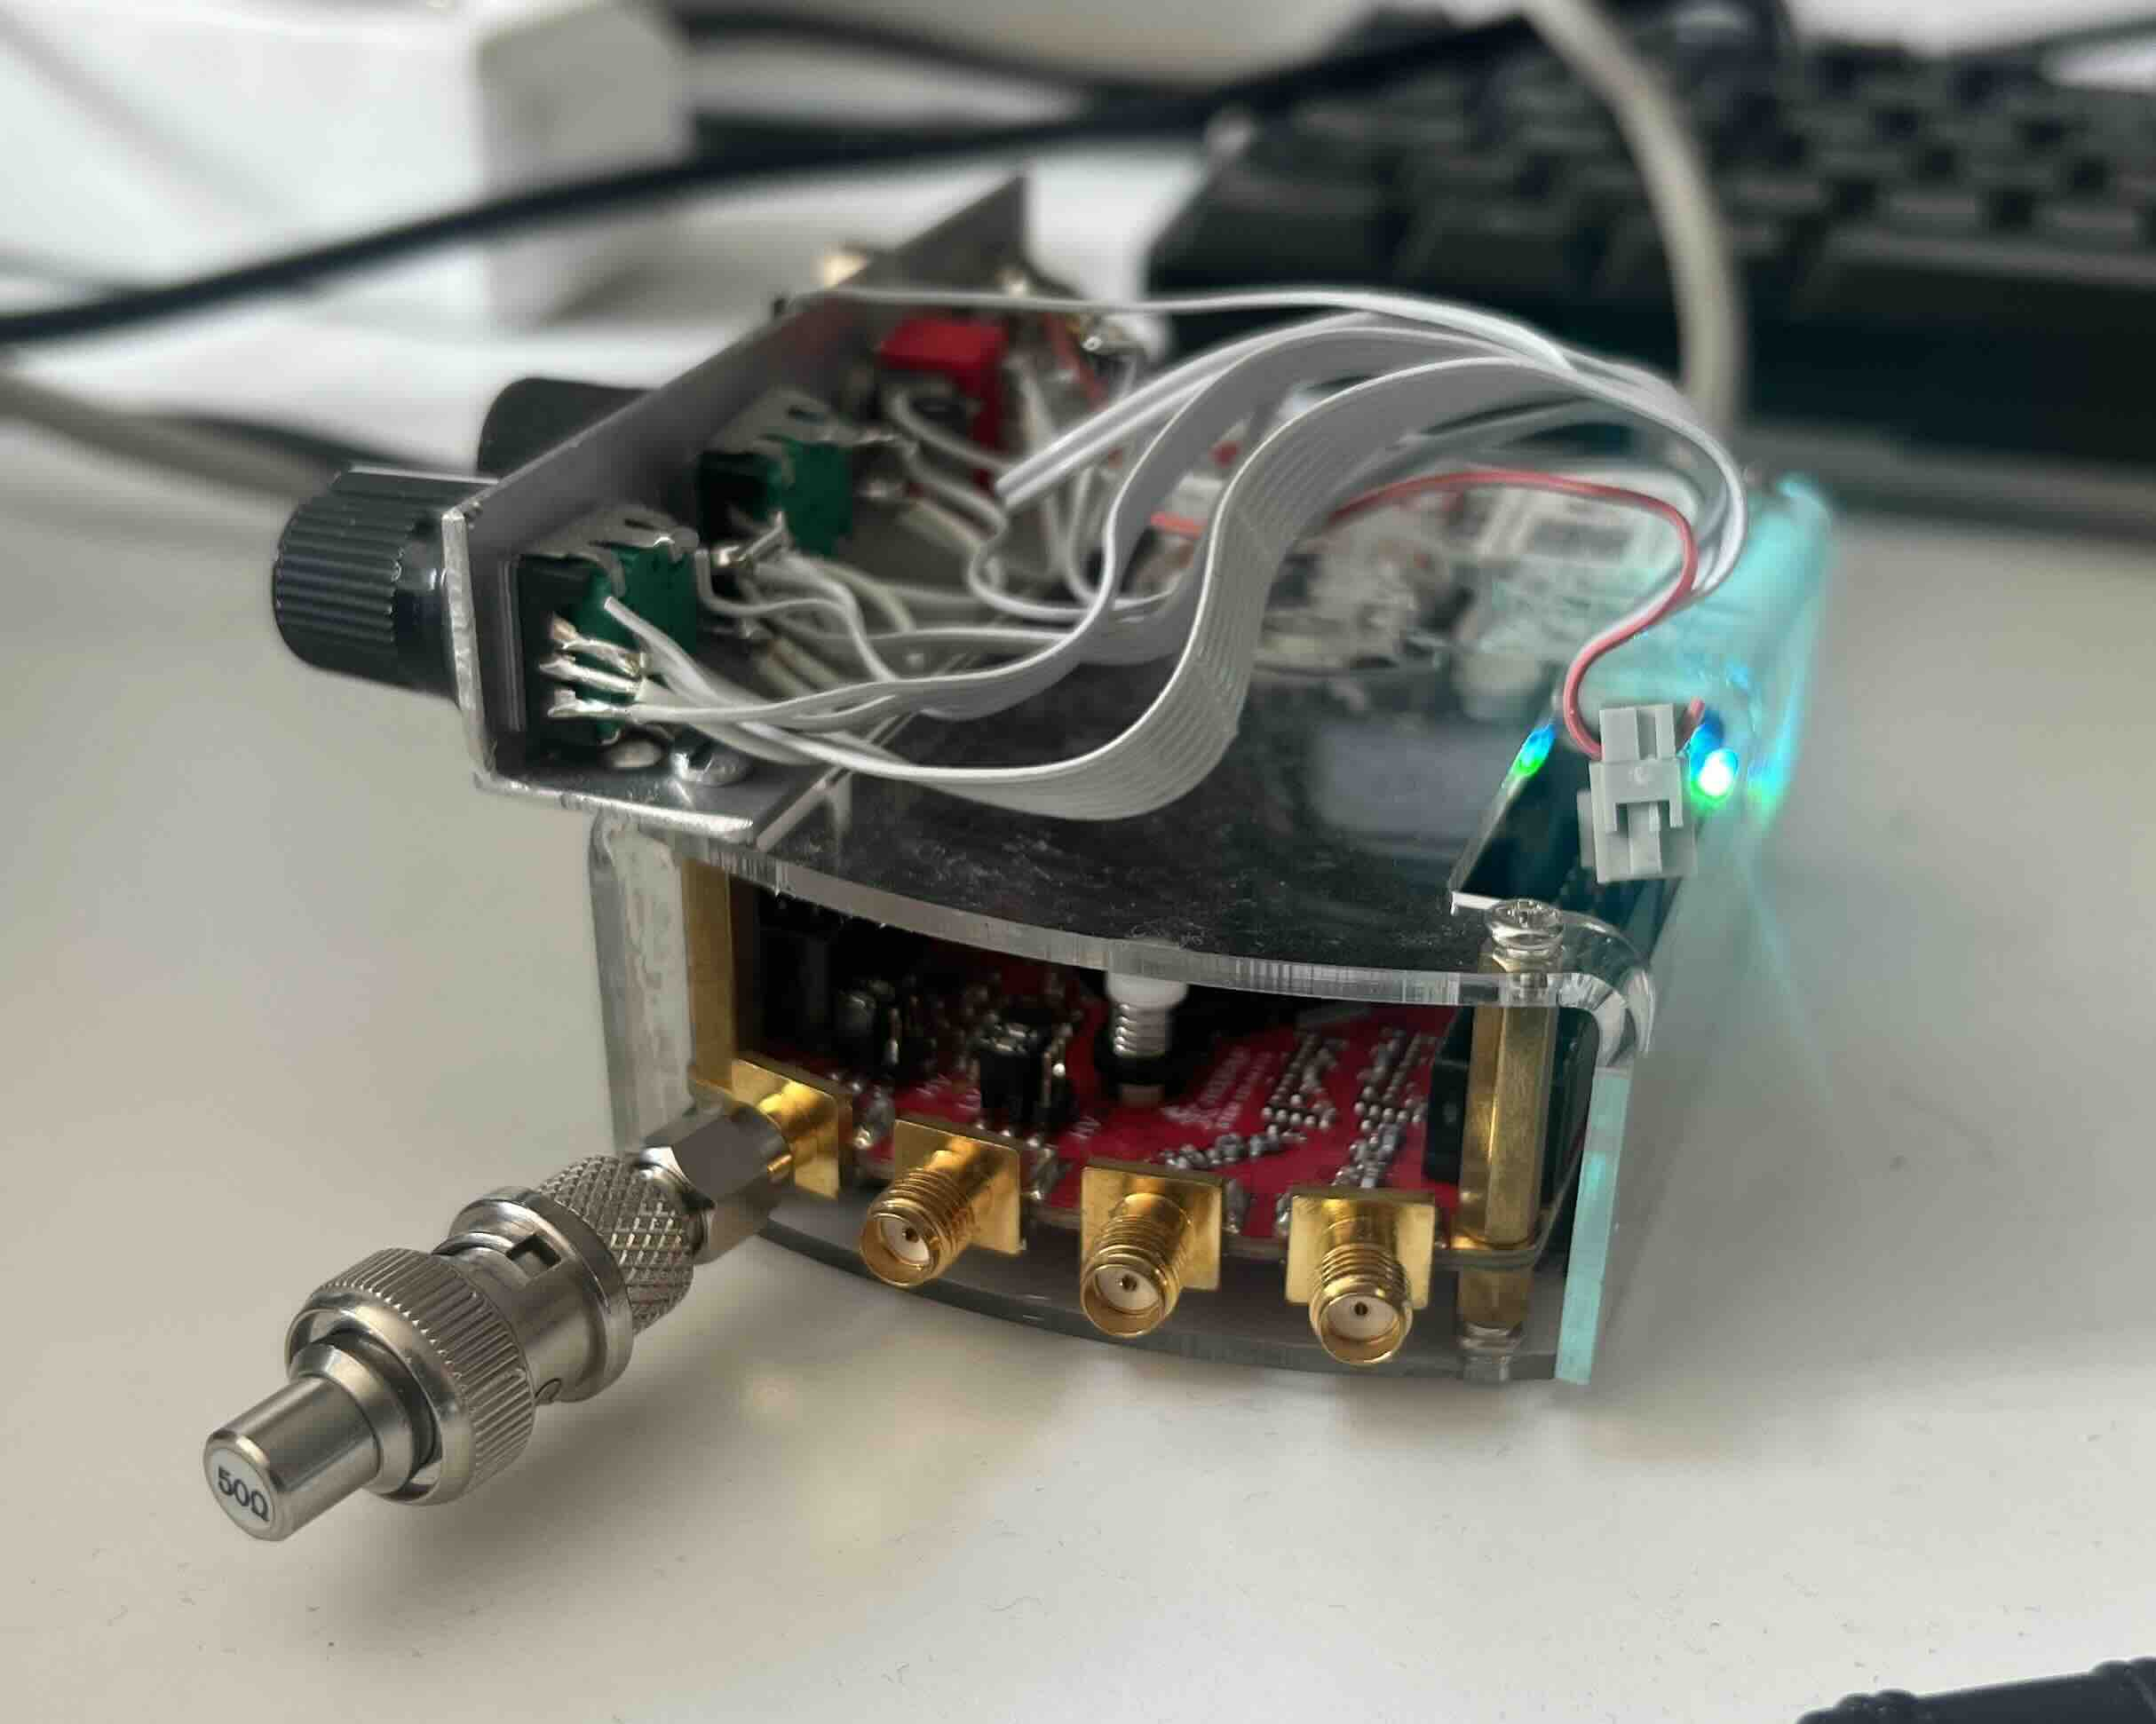
\includegraphics[width=\textwidth]{images/chapter_2/2_noise/noise_resistor.jpg}
        \caption{A 50 $\Omega$ resistor connected to input channel A of the Red Pitaya.}
        \label{fig:ch2_resistor_noise}
    \end{subfigure}
    \hspace{.025\linewidth}
    \begin{subfigure}[t]{0.47\linewidth}
        \centering
        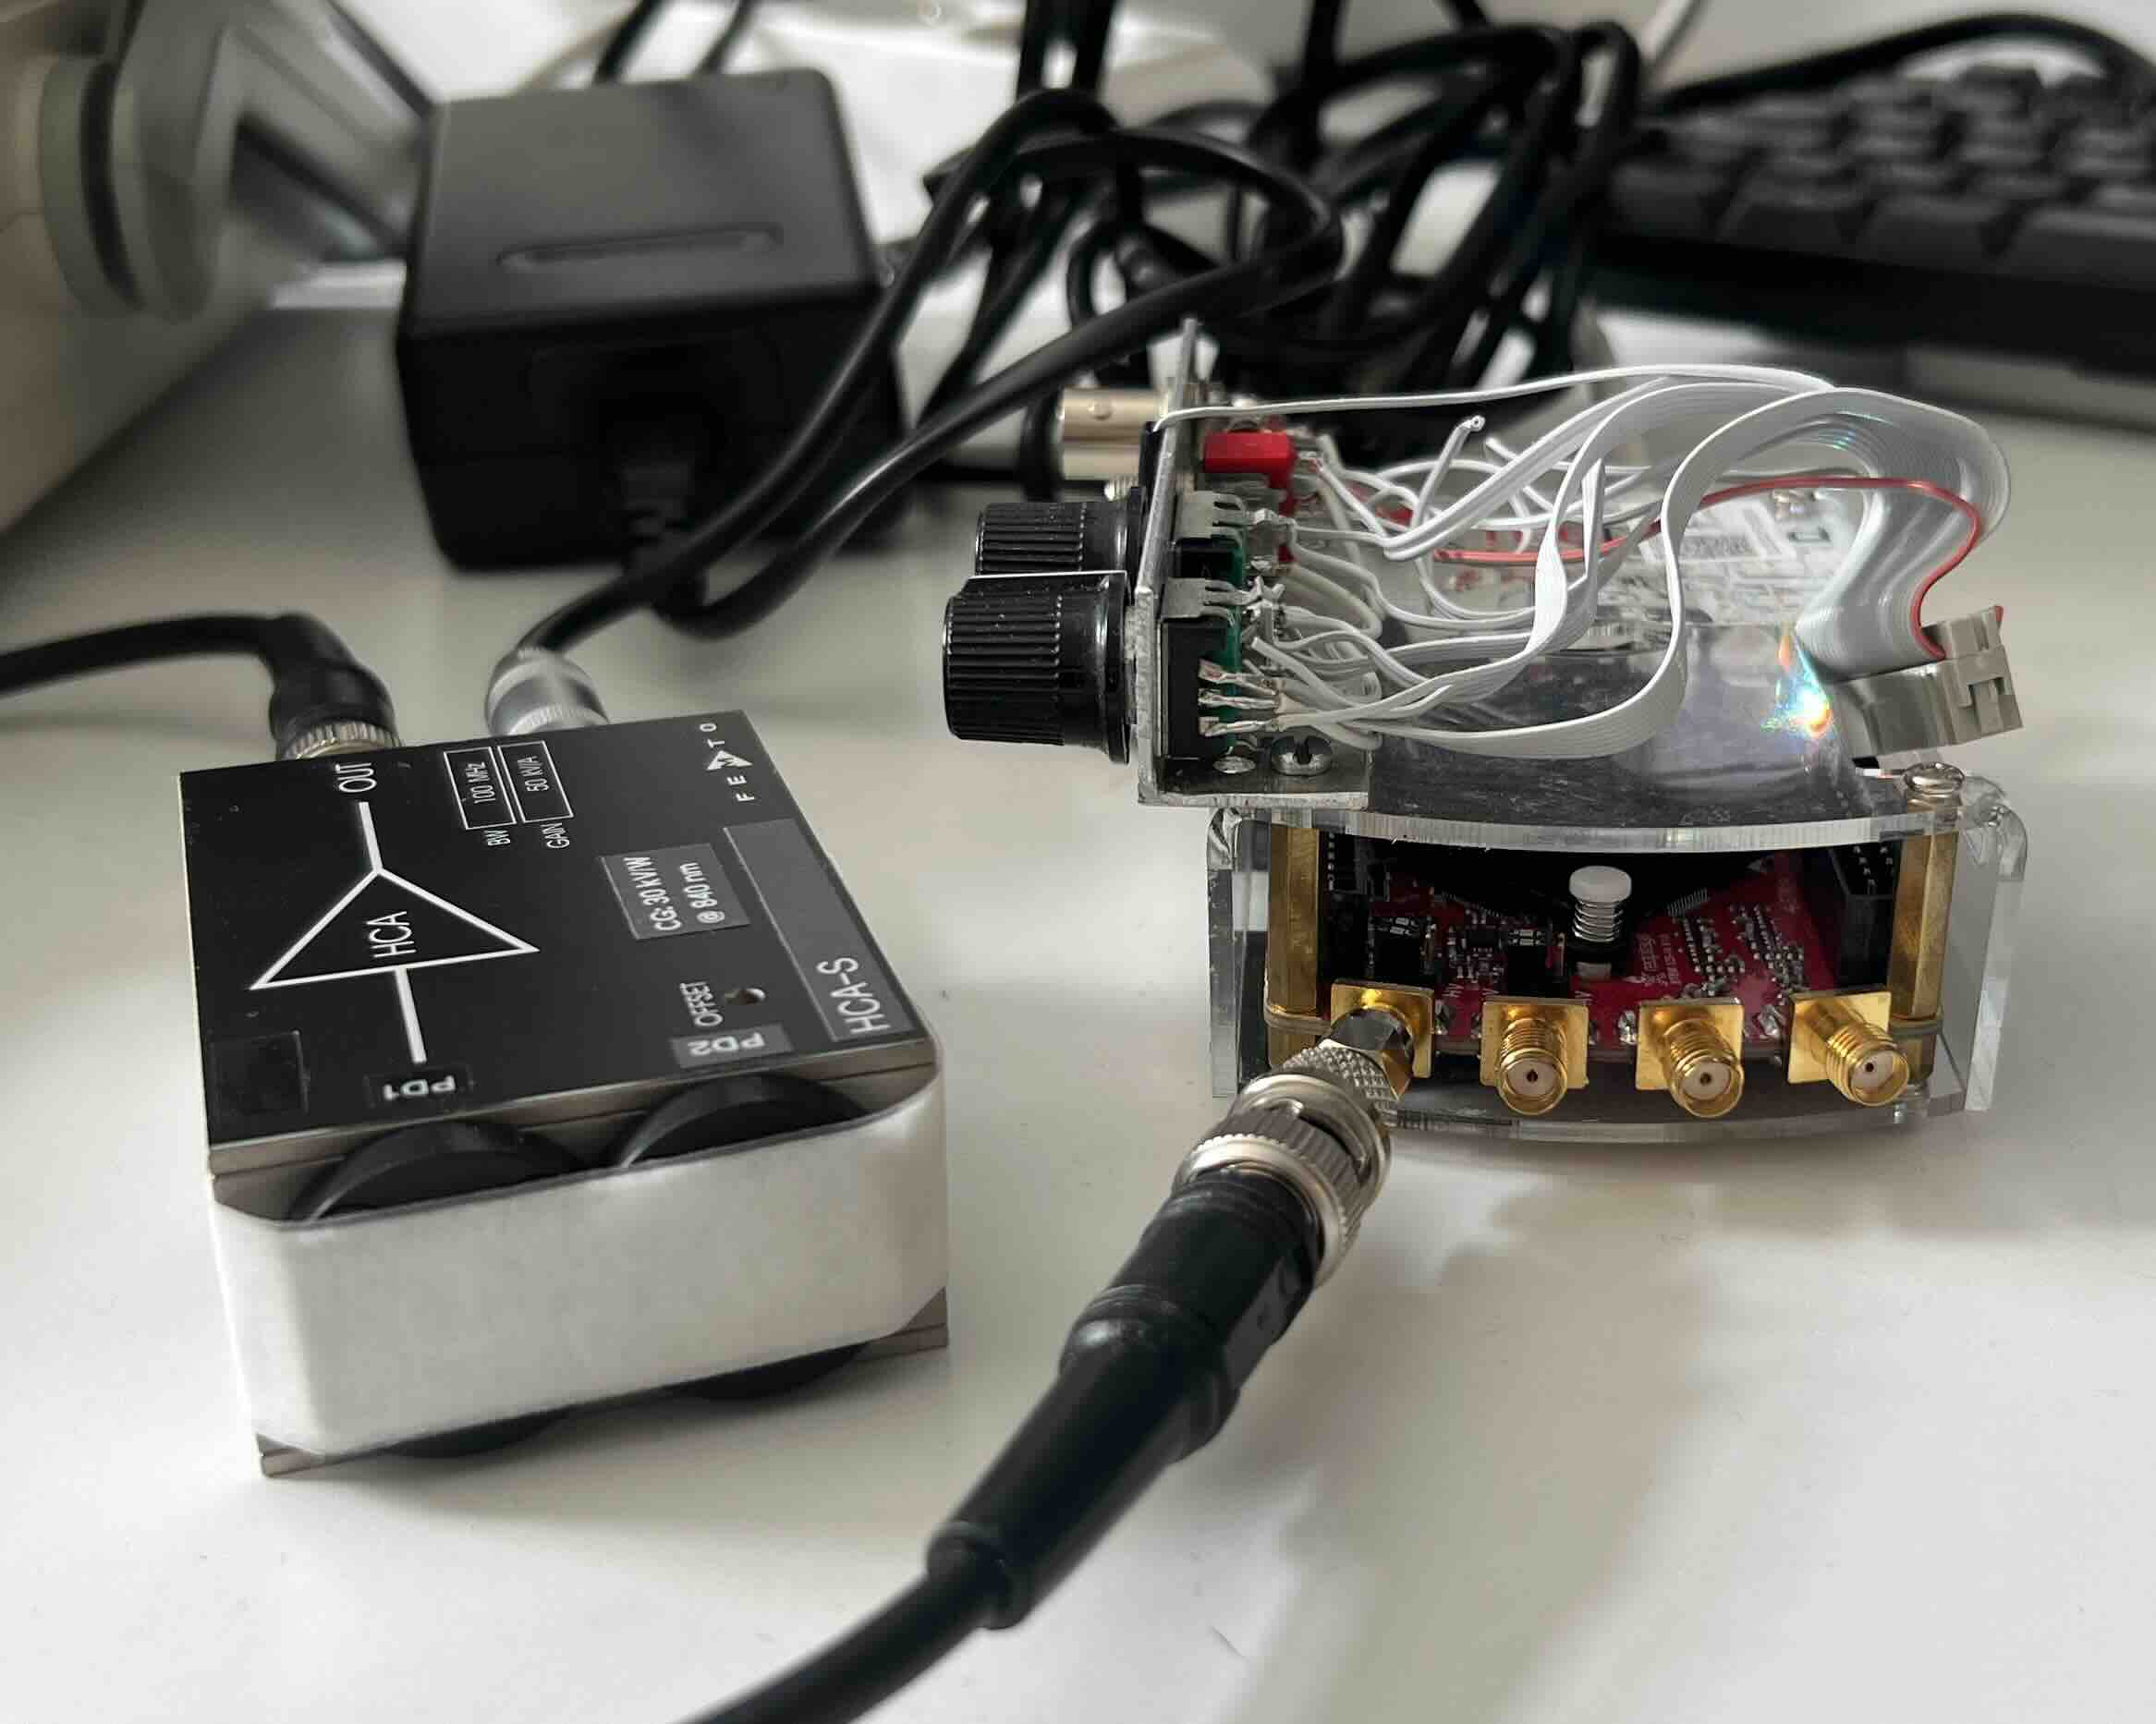
\includegraphics[width=\textwidth]{images/chapter_2/2_noise/noise_homo.jpg}
        \caption{A homodyne detector with inputs taped over connected to input channel A of the Red Pitaya.}
        \label{fig:ch2_homo_noise}
    \end{subfigure}
    \caption{Experimental setups for determining noise levels.}
    \label{fig:ch2_noise_setup}
\end{figure}

\paragraph{Methodology}

To determine the intrinsic device noise of the Red Pitaya, a resistor matching the input impedance of the Red Pitaya (50 $\Omega$) was connected to a selected input channel to block out noise coming from the external environment, as shown in Figure \ref{fig:ch2_resistor_noise}. Similarly, to determine the electronic noise of the homodyne detection system, a homodyne detector with its two inputs (where the beam splitter outputs would enter) taped over was connected to a selected input channel of the Red Pitaya, as shwon in Figure \ref{fig:ch2_homo_noise}. For each test scenario, using Deep Memory Acquisition, N = 524,288 samples of noise signal data were extracted for processing and analysis via remote SCPI commands.

%%%%%%%%%%%%%%%%%%%%%%%%%%%%%%%%%%%%%%%%%%%%%%%%%%%%%%%%%%%%%%%%%%%%%%%%%%%%%%%%
\subsubsection{Data Analysis}

\begin{figure}[ht]
    \centering
    \begin{subfigure}[t]{0.48\linewidth}
        \centering
        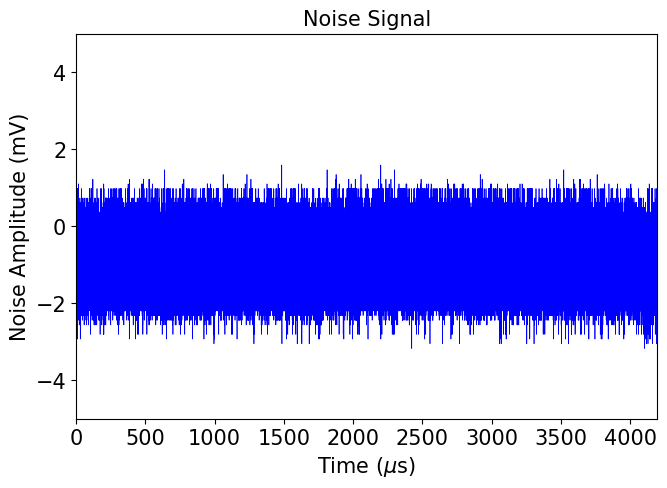
\includegraphics[width=\textwidth]{images/chapter_2/2_noise/signal.png}
        \caption{}
        \label{fig:ch2_signal}
    \end{subfigure}
    \hspace{.025\linewidth}
    \begin{subfigure}[t]{0.48\linewidth}
        \centering
        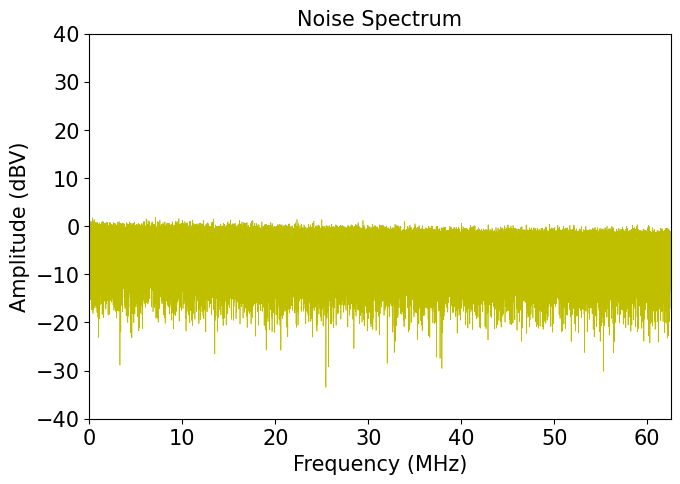
\includegraphics[width=\textwidth]{images/chapter_2/2_noise/spectrum.png}
        \caption{}
        \label{fig:ch2_spectrum}
    \end{subfigure}
    \caption{Signal and spectrum of Red Pitaya's intrinsic noise.}
    \label{fig:ch2_intrinsic}
\end{figure}

Figure \ref{fig:ch2_signal} shows the intrinsic device noise of the Red Pitaya sampled over 4194 $\mu$s (max ADC rate of 125 MHz for N = 524,288 samples). This set of noise data was converted to noise spectrum as shown in Figure \ref{fig:ch2_spectrum} using Numpy FFT (Fast Fourier Transform) functions. The noise spectrum was cut off at the Nyquist frequency and the amplitude converted to decibel-volts for better visualization. The absence of sharp peaks across the frequency range of the noise spectrum assured that the Red Pitaya is not intrinsically hypersensitive to any particular signal frequencies.

The noise signal histogram of the Red Pitaya and the homodyne detection system were also produced and are shown in Figure \ref{fig:ch2_distribution}. The histograms are fitted with Gaussian distribution curves using SciPy and the variances were extracted from the fit where $\sigma_\text{RPN} = 0.54$ mV. The extracted $\sigma_\text{RPN}$ is within the same order of magnitude of the value provided by the manufacturer, which is 0.45 mV \cite{rp}. Additionally, we have that $\sigma^2_\text{HDN} + \sigma^2_\text{RPN} = (5.41 \text{mV})^2$. This implies that $\sigma_\text{HDN} = 5.28\ \text{mV} \gg \sigma_\text{RPN}$, i.e. the Red Pitaya is much less noisy compared to the homodyne detector, which is ideal for the experiment.

\begin{figure}[ht]
    \centering
    \begin{subfigure}[t]{0.47\linewidth}
        \centering
        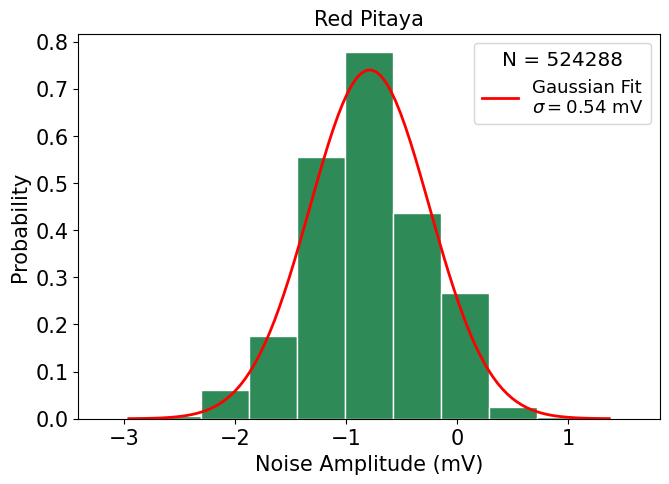
\includegraphics[width=\textwidth]{images/chapter_2/2_noise/distr_rp.png}
        \caption{}
        \label{fig:ch2_signal_distr}
    \end{subfigure}
    \hspace{.025\linewidth}
    \begin{subfigure}[t]{0.48\linewidth}
        \centering
        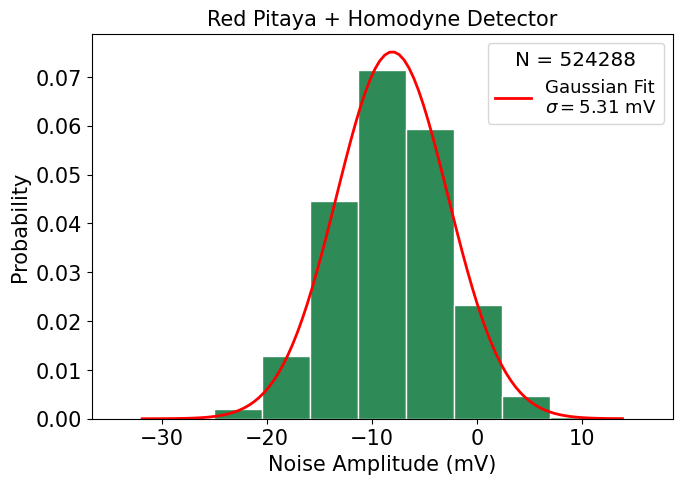
\includegraphics[width=\textwidth]{images/chapter_2/2_noise/distr_homo.png}
        \caption{}
        \label{fig:ch2_spectrum_distr}
    \end{subfigure}
    \caption{Noise signal distribution of (a) the Red Pitaya with a 50 $\Omega$ resistor connected to input and (b) the homodyne detection system with Red Pitaya.}
    \label{fig:ch2_distribution}
\end{figure}

\paragraph{Conclusion}

The Red Pitaya noise signal study suggests that the Red Pitaya is a viable candidate for data acquisition within the homodyne detection system with regards to noise sensitivity. This is shown by the absence of sharp frequency spikes in the intrinsic noise spectrum of the Red Pitaya. On top of that, the fact that the Red Pitaya is $\sim 10$ times less noisy than the homodyne detector, means the shot noise limit of the entire homodyne detection system can be kept at an ideally low value.